\documentclass[tikz,border=2mm]{standalone}
\usetikzlibrary{positioning}
\begin{document}
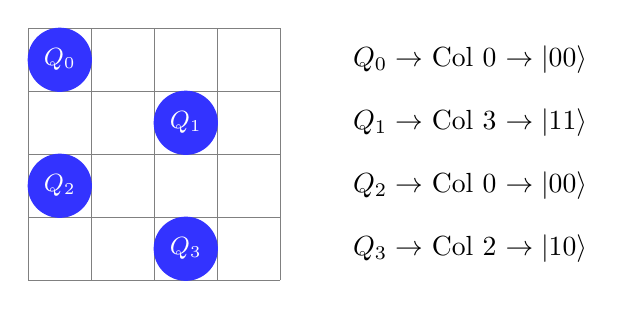
\begin{tikzpicture}[
    queen/.style={circle, fill=blue!80, text=white, minimum size=0.5cm, font=\bfseries\small}
]
\draw[step=0.8cm,gray,very thin] (0,0) grid (3.2,3.2);
\node at (0.4, 3.2-0.4) [queen] {$Q_0$};
\node at (1.2+0.8, 3.2-1.2) [queen] {$Q_1$};
\node at (0.4, 3.2-2.0) [queen] {$Q_2$};
\node at (0.4+1.6, 3.2-2.8) [queen] {$Q_3$};

\node[anchor=west] at (4, 2.8) {$Q_0 \rightarrow$ Col 0 $\rightarrow |00\rangle$};
\node[anchor=west] at (4, 2.0) {$Q_1 \rightarrow$ Col 3 $\rightarrow |11\rangle$};
\node[anchor=west] at (4, 1.2) {$Q_2 \rightarrow$ Col 0 $\rightarrow |00\rangle$};
\node[anchor=west] at (4, 0.4) {$Q_3 \rightarrow$ Col 2 $\rightarrow |10\rangle$};
\end{tikzpicture}
\end{document}
